\chapter{Lecture 21 - Fuel Thermal Conductivity Model}
\label{ch:ch21}
\section{Objectives}
The objectives of this lecture are:
\begin{enumerate}
\item Analyze the heat equation taking into account temperature-dependent thermal conductivity.
\item Present a current fuel thermal conductivity model.
\item Carry out an example calculation using a graphical technique
\end{enumerate}

\section{The Heat Equation, Revisited}

This being a lecture about thermal conductivity models, we should first start with the heat equation.

\begin{equation}
\rho c_p \frac{\partial T}{\partial t} = S + \nabla \cdot k \nabla T
\label{eq:heat_eq}
\end{equation}
where, as a reminder, $\rho$ is the mass density, $c_p$ is the material specific heat, $T$ is temperature, $t$ is time, $S$ is a volumetric heat source term, and $k$ is the material thermal conductivity.

This model will be applied to cylindrical fuel pins that are typical for a nuclear reactor core; accordingly we will specify the cylindrical coordinate system for the $\nabla$ operator.  If we further assume steady state, Equation \ref{eq:heat_eq} becomes:
\begin{align}
\rho c_p  \cancelto{0}{\frac{\partial T}{\partial t}} &= q^{\prime \prime \prime} + \frac{1}{r} \frac{\partial}{\partial r}\left(k r \frac{\partial T}{\partial r}\right)+ \frac{1}{r^2} \frac{\partial}{\partial \phi} \left(k \frac{\partial T}{\partial \phi} \right) + \frac{\partial}{\partial z}\left(k \frac{\partial T}{\partial z} \right) \nonumber \\
0 &= q^{\prime \prime \prime} + \frac{1}{r} \frac{\partial}{\partial r}\left(k r \frac{\partial T}{\partial r}\right)+ \frac{1}{r^2} \cancelto{0}{\frac{\partial}{\partial \phi} \left(k \frac{\partial T}{\partial \phi} \right)} + \cancelto{0}{\frac{\partial}{\partial z}\left(k \frac{\partial T}{\partial z} \right)} \nonumber \\
0 &= q^{\prime \prime \prime} r + \frac{\partial}{\partial r} \left(kr \frac{\partial T}{\partial r} \right)
\label{eq:heat_simplified}
\end{align}
where derivatives in $\phi$ are assumed zero due to radial symmetry and the derivative of temperature with respect to $z$ is assumed to be zero since most of the heat is conducted in the radial direction.\marginnote{\textbf{Note:} This last assumption is quite true near the axial center of the fuel pin, far from the top or bottom core boundary.  Near the boundary there is some axial heat conduction and this assumption is not quite as good.}  The equation is now an second-order \emph{ordinary} differential equation\sidenote{We have just assumed-away any dependence on independent variables other than $r$.} with a non-homogeneous source term that we will, for the purposes of this lecture, take to be a constant.  

If we integrate both sides of Equation \ref{eq:heat_simplified} we get:
\begin{align}
0 &= q^{\prime \prime \prime} \frac{r^2}{2} + kr\frac{dT}{dr} + c_1 \nonumber \\
0 &= q^{\prime \prime \prime} \frac{r}{2} + k\frac{dT}{dr} + \frac{c_1}{r} 
\label{eq:heat_simplified2}
\end{align}
where $c_1$ is a constant that must be found from the boundary conditions.\marginnote{In Equation \ref{eq:heat_simplified2} we divided through by $r$ to put the equation into a more standard form.  We might also have divided through by $k$ so that the coefficient for the highest derivative of $r$ is equal to 1 - that would have really been the standard form - but for purposes of this lecture we will leave the $k$ where it is.} 

At this point in the analysis we will introduce an additional complexity that we have been able to safely ignore up until now; namely we will assume that $k$ is a function of material temperature, $k(T)$.  Inserting this new notation into our equation and re-arranging gives us:

\begin{equation}
-k(T) \ \frac{dT}{dr} = \frac{q^{\prime \prime \prime}}{2} r + \frac{c_1}{r}
\label{eq:heat_simplified3}
\end{equation}

This equation is now non-linear but, thankfully is separable; we can formally move $\partial r$ from the ``denominator'' on the right hand side to get:

\begin{equation}
-\int_{T(r=0)}^{T(r=R)} k(T) \ dT = \int_{r = 0}^{r = R} \frac{q^{\prime \prime \prime}}{2} r + \frac{c_1}{r} \ dr = \frac{q^{\prime \prime \prime}R^2}{4} + c_1 \ln(r) \Big|_0^R
\label{eq:heat_simplified4}
\end{equation}
where, in order for the right hand side of Equation \ref{eq:heat_simplified4} to remain bounded as $r\rightarrow 0$, $c_1$ must be set equal to zero. We've kept the left hand side as it is, for the time being, until we can specify the form of $k(T)$.  

The last manipulations we will do are cosmetic in nature: on the left hand side we will flip the interval of integration to remove the minus sign; on the right hand side we observe that $q^{\prime \prime \prime} \pi R^2 L = q^{\prime}L$ to give us:
\begin{equation}
\int_{T(R)}^{T(0)} k(T) \ dT = \frac{q^{\prime}}{4 \pi}
\label{eq:heat_simplified_final}
\end{equation}
where it is expected that $T(R)$ would be given as a boundary condition.
 
It would be a stretch to call this a ``solution'' to Equation \ref{eq:heat_eq}; we have not derived an expression for temperature as a function of radius.  What we have is a way to determine the temperature at the center-line of the fuel---the maximum fuel temperature $T_{\text{max}}$---given a constant linear heat rate, $q^{\prime}$, and a formula for $k(T)$. What we hope to do is find the value of $T(0)$ so that the integral on the left of Equation \ref{eq:heat_simplified_final} is equal to the constant computed on the right.  Alternatively we might assume a maximum permissible fuel center line temperature and solve for the corresponding linear heat rate, fuel surface heat flux, or volumetric heat generation rate.\sidenote{These last two would also require that you specify the fuel pin outer radius.}

\section{FRAPCON Fuel Thermal Conductivity Model} \index{FRAPCON, model}
The standard model to use for uranium oxide and mixed oxide nuclear fuel is the FRAPCON-3 model established from empirical data and maintained by Pacific Northwest National Laboratory.\cite[-2.0cm]{lanning2005frapcon} The model captures changes to thermal conductivity due to the following factors:
\begin{marginfigure}
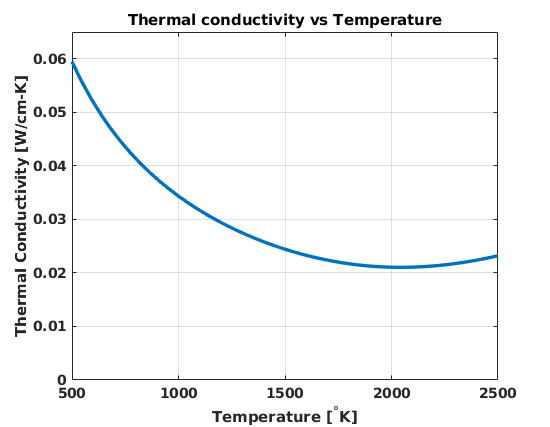
\includegraphics{uo2_k_vs_T.png}
\caption{Thermal conductivity for unirradiated $\text{UO}_2$ at 95\% theoretical density using the FRAPCON model.}
\label{fig:uo2_vs_T}
\end{marginfigure}

\begin{marginfigure}
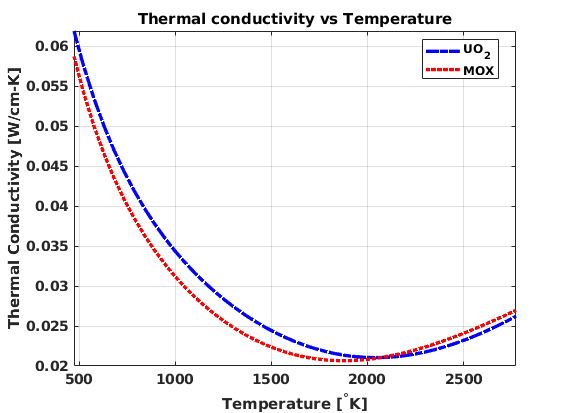
\includegraphics{uo2_and_mox_vs_T.png}
\caption{Comparison of $\text{UO}_2$ and MOX thermal conductivity.}
\label{fig:uo2_and_mox_vs_T}
\end{marginfigure}

\begin{marginfigure}
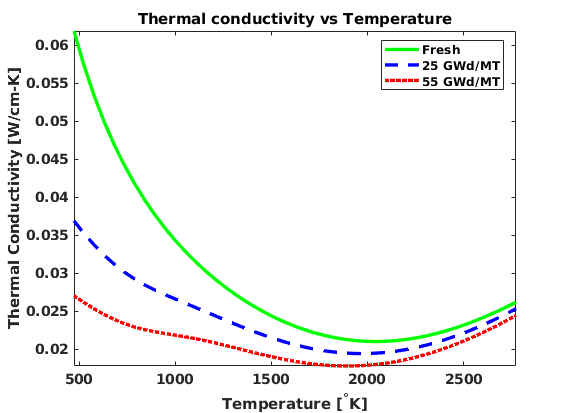
\includegraphics{uo2_burnup.png}
\caption{Impact of burn-up on $k$ for UO$_{2}$.}
\label{fig:uo2_burnup}
\end{marginfigure}

\begin{itemize}
\item \textbf{Temperature.} For many materials, increase in temperature results in a decrease in thermal conductivity.  As can be seen in Figure \ref{fig:uo2_vs_T}, this is true for oxide fuels below 1750$^{\circ}$C but above that temperature thermal conductivity increases slightly.   
\item \textbf{$\text{UO}_2$ vs Mixed Oxides.}  Adding a mixture of plutonium oxides along with uranium oxides results in lower thermal conductivity over most temperatures.  This behavior is shown in Figure \ref{fig:uo2_and_mox_vs_T}.  Generally speaking the more complex behavior of thermal conductivity of MOX fuel adds to the list of issues to address when transitioning to a closed fuel cycle where plutonium produced in reactors is consumed as fuel.
\item \textbf{Burn-up.}  The overall effect on thermal conductivity is due to a number of phenomena that all occur during core life including changes in the porosity, composition and stoichiometry of the fuel.  Generally, as burn-up increases, the thermal conductivity of the fuel decreases.  This is shown for $\text{UO}_2$ fuel in Figure \ref{fig:uo2_burnup}.  
\item \textbf{Density.} Generally, increasing UO$_{2}$ density increases thermal conductivity with the converse effect for reduced density.  The effect of density on thermal conductivity is shown quantitatively in Figure \ref{fig:uo2_density}.
\end{itemize}

\begin{marginfigure}
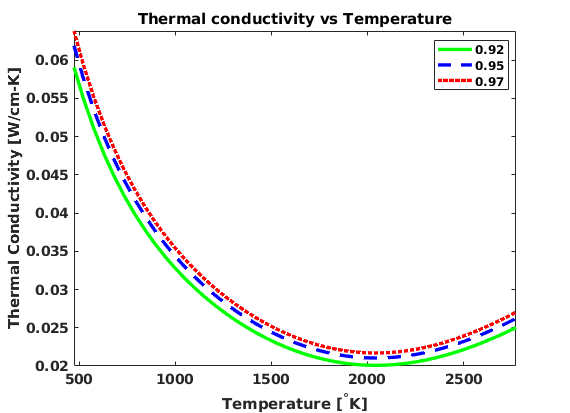
\includegraphics{uo2_density.png}
\caption{Impact of density on thermal conductivity for UO$_{2}$.}
\label{fig:uo2_density}
\end{marginfigure}

All of these effects are captured in the FRAPCON model for thermal conductivity.  The model is as shown in Equation \ref{eq:FRAPCON}


\begin{multline}
k_{0.95 \ \text{TD}} = \left\{A + BT + a \cdot \text{gad} + f(Bu) +  \left[1-0.9e^{-0.04 Bu} \right]g(Bu)h(T) \right\}^{-1} \\ + \frac{E}{T^2}e^{-\sfrac{F}{T}}
\label{eq:FRAPCON}
\end{multline}

where the following constants and functions are defined:
\begin{itemize}
\item a = 115.99 [cm-K/W]
\item $Bu$ is burn-up given in MWd/kg or GWd/MT
\item f($Bu$) = $0.187\times $Bu [cm-K/W].  This is intended to capture the effect of fission products in the fuel crystal matrix.
\item gad = gadolinium weight percent
\item $h(t) = \left[1 + 396 e^{-\sfrac{Q}{T}} \right]^{-1}$.  This term captures the temperature dependence of annealing of irradiation defects.
\item Q = 6380$^{\circ}$K, temperature of annealing parameter.
\item T = temperature, given in Kelvin.
\end{itemize}
The constants $A$, $B$, $E$, and $F$ are given in Table \ref{tab:FRAP_constants}; the value of $x$ for the (U,Pu)O$_2$ material correlations is defined by: $x = 2.0 - \text{O/M}$, where O/M is the oxygen-to-metal atomic ratio in the fuel material.

\begin{margintable}
\begin{tabular}{l c c}
\toprule
   & UO$_2$ & (U,Pu)O$_2$ \\
\midrule
A [cm-K/W] & 4.52 & $285x+3.5$ \\
B [cm/W] & $2.46 \times 10^{-2}$ & $\left(2.86 - 7.15x\right)\times 10^{-2}$ \\
E [ W-K/cm] & $3.5\times 10^7$ & $1.5\times 10^7$ \\
F [K] & 16,361 & 13,520 \\
\bottomrule
\end{tabular}
\caption{Values of constants in FRAPCON correlations for thermal conductivity.}
\label{tab:FRAP_constants}
\end{margintable}
The resulting thermal conductivity $k_{0.95 \ \text{TD}}$ is given in W/cm-K for oxide fuel at 95 percent of theoretical density.  If the fuel density is something different than 95 percent of theoretical density, a correction factor must be applied; this is given by Equation \ref{eq:FRAP_density}.


\begin{equation}
\eta(\rho) = \frac{1.0789 \sfrac{\rho}{\rho_{\text{TD}}}}{1 + 0.5\left(1 - \sfrac{\rho}{\rho_{\text{TD}}} \right)} 
\label{eq:FRAP_density}
\end{equation}

so that $k(\rho) = \eta(\rho)k_{0.95 \ \text{TD}}$. In total, therefore, thermal conductivity is a function of temperature, density, gadolinium concentration and burn-up for either UO$_2$ or (U,Pu)O$_2$ fuel.  We could re-write Equation \ref{eq:heat_simplified_final} reflecting this as shown in the equation below:

\begin{equation}
\int_{T(R)}^{T(0)} k(T,gad,Bu)\eta(\rho) \ dT = \frac{q^{\prime}}{4 \pi}
\label{eq:heat_final}
\end{equation}
Analytically solving this equation is not something we are interested in pursuing. In the next section, we will use a ``graphical-method'' to solve the problem; in the next lecture we will discuss how you can use MATLAB to solve Equation \ref{eq:heat_final}.

\section{Example Calculation - Graphical Method}

Consider a PWR core operating at full power with a fuel pin linear heat rate of 25 kW/m.  Temperature of the fuel outer surface is 400$^{\circ}$C. Assume the fuel pin was initially loaded with 5 w/o gadolinium for reactivity control.  Using the FRAPCON-3 model incorporated into Figure \ref{fig:integral_fuel_thermal_conductivity}, estimate the temperature at the center of the fuel pin at:
\begin{enumerate}
\item beginning of life;
\item burn-up of 25 MWd/kg; and
\item burn-up of 55 MWd/kg
\end{enumerate}

\begin{marginfigure}
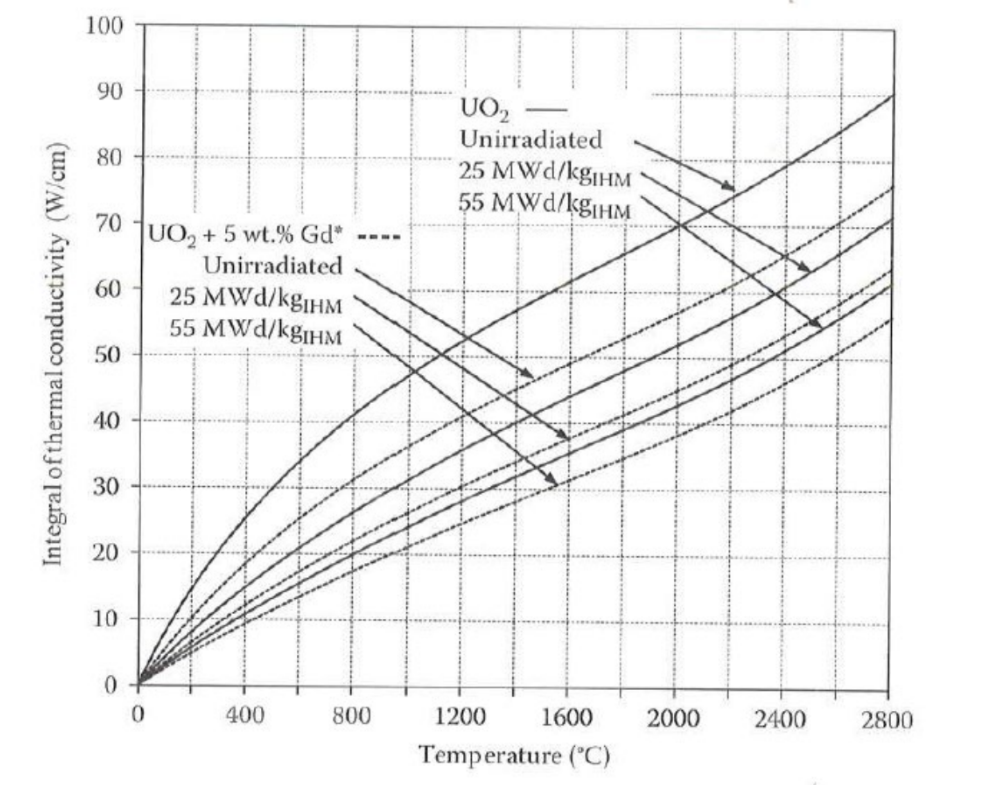
\includegraphics{integral_of_fuel_thermal_conductivity.png}
\caption{Integral of fuel thermal conductivity.}
\label{fig:integral_fuel_thermal_conductivity}
\end{marginfigure}

To solve these problems we need to a) select the correct curve corresponding to burn-up and gadolinium concentration; b) use the given linear heat rate to calculate the right-hand-side of Equation \ref{eq:heat_final}; and c) use the curve as shown below.

Using the graph, we can evaluate:
\begin{equation}
\int_{T(R)}^{T(0)} k(T,gad,Bu)\eta(\rho) \ dT = K(T(0)) - K(T(R)) = \frac{q^{\prime}}{4 \pi}
\label{eq:heat_integrated}
\end{equation}
where $K(T)$ the integral of the thermal conductivity evaluated to temperature $T$.

\begin{marginfigure}
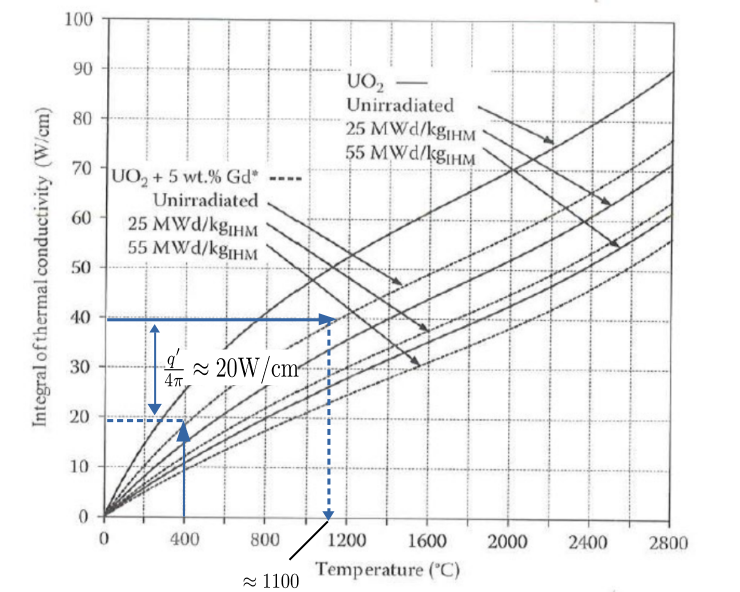
\includegraphics{fuel_k_graphical_part_a.png}
\caption{Using graphical method for fuel thermal conductivity; part 1.}
\label{fig:fuel_graphical_part_a}
\end{marginfigure}
For the first problem we select the top dashed line corresponding to unirradiated UO$_2$ fuel with 5 w/o Gd; we evaluate the integral of the thermal conductivity at the fuel outer surface temperature of 400$^{\circ}$C and get a result just under 20 W/cm.  This is illustrated in Figure \ref{fig:fuel_graphical_part_a}.  We do not know $T(0)$ yet but we can calculate the right hand side of Equation \ref{eq:heat_integrated} from the given linear heat rate; $\frac{q^{\prime}}{4 \pi} = \frac{250 \text{W/cm}}{4 \pi} = 19.9 \text{W/cm}$.\sidenote{\textbf{Note:} Pay attention to units for the given linear heat rate and thermal conductivity.} So even if we do not know $T(0)$, we know that $K(T(0)) - K(T(R)) \approx 20 \text{W/cm}$, so we just need to find where the top dashed curve giving the integral of thermal conductivity intersects with, roughly, $20 + 20 = 40 \text{W/cm}$.  We read the corresponding temperature and its about 1100$^{\circ}$C.

Parts 2 and 3 are done in the same way; we simply need to use different thermal conductivity curves corresponding to 25 MWd/kg and 55 MWd/kg burn-up. The graphical solutions to the second and third problems are shown in Figure \ref{fig:fuel_graphical_part_b} and Figure \ref{fig:fuel_graphical_part_c}.

\begin{marginfigure}
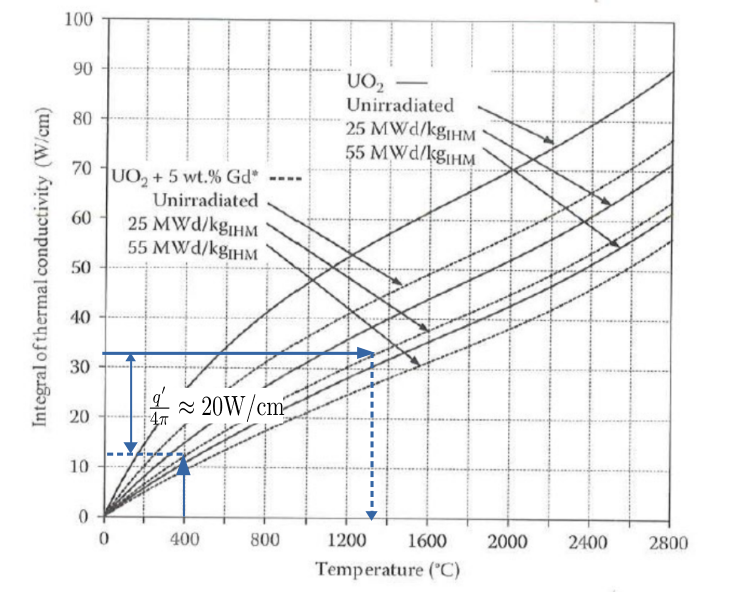
\includegraphics{fuel_k_graphical_part_b.png}
\caption{Using graphical method for fuel thermal conductivity; part 2.}
\label{fig:fuel_graphical_part_b}
\end{marginfigure}

\begin{marginfigure}
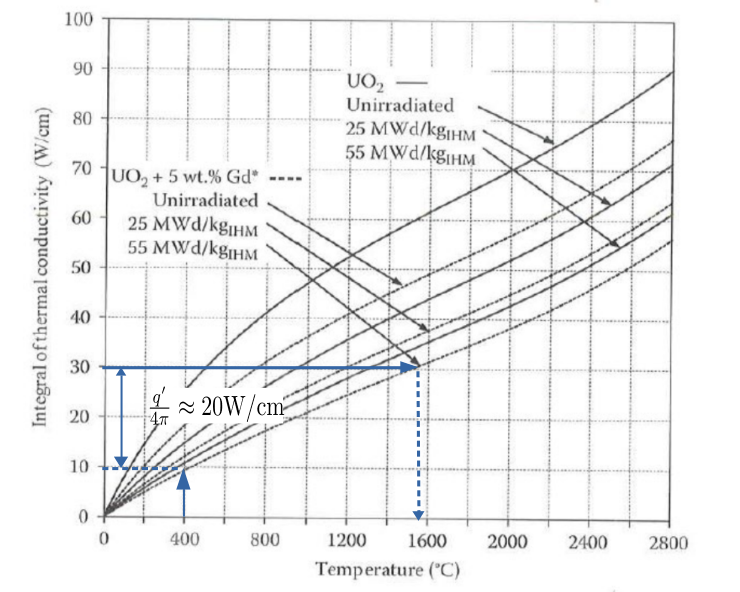
\includegraphics{fuel_k_graphical_part_c.png}
\caption{Using graphical method for fuel thermal conductivity; part 3.}
\label{fig:fuel_graphical_part_c}
\end{marginfigure}
Note that as burn-up increases, fuel thermal conductivity decreases, and for the same linear heat rate and external fuel temperature, the center line temperature of the fuel increases.  This should correspond with what you expect to see for system response to decreasing fuel thermal conductivity.

